%!TEX root = ../terrainbook.tex
% chktex-file 46

\setchapterpreamble[u]{\margintoc}
\graphicspath{{gdem/figs/}}


\chapter{Global digital elevation models}% or global terrains
\label{chap:gdem}

We define as ``global digital elevation models'' (or global terrains; we refer to them as ``gDEMs'' in this book) the datasets that cover (most of) the Earth.%
\index{global DEM}
Those datasets require different acquisition methods from local datasets, since flying an airplane or performing local surveys at the scale of the Earth has not been done yet, and it would be prohibitively expensive.
The acquisition instruments for a global coverage must be \emph{space-borne}, \ie\ mounted on a satellite for instance.
Notice that the orbit of some satellites makes them technically non-global, but that we still refer to their datasets as global since they have a wide coverage, just restricted to certain latitudes.

%

It cannot be understated that before the introduction of gDEMs (with SRTM v1 in 2000, see below for more information), we had no way of knowing the elevation for a given location on the Earth.
Indeed, looking at the datasets listed and/or hosted at
\marginnote{\url{https://opentopography.org}}
OpenTopography (Figure~\ref{fig:dem_coverage}), we can observe that, even in 2022, local elevation datasets are mostly limited to developed countries.
\begin{figure}
  \centering
  \includegraphics[width=\linewidth]{opentopography.pdf}
  \caption{OpenTopography coverage with some European datasets added in pink; there are in fact more European datasets but there is no global registry for them.}%
  \label{fig:dem_coverage}
\end{figure}

%

Global DEMs enable us to perform \emph{global} environmental studies, such as geological studies, hydrological modelling, ecosystems dynamics, the understanding of volcanic processes, and flow simulations (see Chapter~\ref{chap:runoff}).

%

While gDEMs are elevation models like local ones (and can be modelled with essentially the same formats and tools as local ones), they have several properties and characteristics that apply only to them, and we report in this chapter on the main ones.

% We first describe global acquisition techniques, then we discuss the properties (and errors and biases, etc.) that the datasets collected will have,


%%%%%%%%%%%%%%%%%%%%
%
\section{Acquisition of global elevation data}[Acquisition of global data]

The acquisition of gDEMs requires the use of a sensor mounted on a satellite.
The three most used instruments to collect elevation information are:
\begin{enumerate}
  \item Photogrammetry from optical satellite images
  \item Interferometric synthetic-aperture radar (InSAR)
  \item Lidar
\end{enumerate}


%%%
\subsection{Photogrammetry from high-resolution satellite images}

See Section~\ref{sec:photogrammetry}.


%%%
\subsection{InSAR}%
\index{InSAR}

The first gDEM (SRTM v1) was collected with InSAR in 2000, aboard the Space Shuttle Endeavour.
As InSAR requires two images of the same area for stereoscopy to derive a DEM, the Shuttle was equipped with two antennas, one in the payload bay, and one on a mast protruding \qty{60}{m} from the Shuttle.

Similarly, the TerraSAR-X satellite was joined by TanDEM-X in 2010, a twin satellite orbiting only a few hundred meters (!) away, to generate InSAR data in a single pass.

See Section~\ref{sec:insar} for more information.


%%%
\subsection{Spaceborne lidar (ICESat-2 + GEDI)}%
\index{spaceborne lidar}\index{lidar}

Spaceborne lidar is a relatively new technique, and has not yet been used to produce a gDEM\@.
We still include it here because it enables \emph{terrain} elevation measurements globally (vegetation can be filtered out), and we believe it will help us create gDEMs in the near future.

%

Lidar was first used in space on the Apollo missions, and with further technological developments, it has been used extensively from the 1990s onwards.
For example, Mercury, Mars, near-Earth asteroids, and lately again the Moon have been scanned using lidar.
Earth surface elevation lidar measurements have also been developed, often flown on the Space Shuttles.
ICESat was the first Earth-based lidar satellite, launched in 2003, with the primary goal of ice sheet monitoring.
It had an elevation accuracy of several cm and was operational for five years.
Most recently, NASA launched in 2018 two missions measure the elevation of the Earth globally with lidar instruments:

\begin{itemize}
  \item \textbf{ICESat-2}
        \marginnote{\url{https://icesat-2.gsfc.nasa.gov/}}\index{ICESat-2}
        (Ice, Cloud, and Land Elevation Satellite-2) is in a low Earth and polar orbit to investigate ice sheets, it covers the Earth between \ang{-88} and \ang{88} latitude.
        Its instrument to measure altimetry is called \emph{Advanced Topographic Laser Altimeter System} (ATLAS).
        Apart from terrain retrieval, ICESat-2 also measures the surface, such as canopy height, and has many other applications such as measuring bathymetry and estimating biomass.
  \item \textbf{GEDI}
        \marginnote{\url{https://gedi.umd.edu/}}\index{GEDI}
        (Global Ecosystem Dynamics Investigation) is attached to the international space station (ISS) and its primary goal is to investigate global ecosystems.
        It does not have global coverage since it collects measurements only between \ang{51.6} N and \ang{51.6} S.
        GEDI has been combined with TanDEM-X data to produce biomass estimates and with Landsat imagery to produce a global canopy height map.
\end{itemize}
\begin{figure}
  \centering
  \includegraphics[width=\linewidth]{orbit}
  \caption{Ground tracks for three successive orbits of ICESat-2 and GEDI\@. The satellite is a represented by a triangle and past orbits fade out. Note the increased density of ground tracks at the latitude of inclination, as well as the lack of coverage beyond \ang{51.6}~latitude for GEDI.}%
  \label{fig:orbit}
\end{figure}

%

The characteristics of both missions are summarised in Table~\ref{tab:lidarcomparison}
\begin{table*}
  \sisetup{detect-weight=true,detect-inline-weight=math}
  \caption{Key characteristics of GEDI and ICESat-2 missions in comparison with a typical airborne lidar mission.}
  \centering
  \begin{tabular}{l|lll}
    \toprule
                           & ICESat-2                             & GEDI                                   & airborne lidar   \\
    \midrule
    \ type                 & discrete photon                      & full waveform                          & either           \\
    \ main objective       & cryosphere monitoring                & ecosystems                             & ---              \\
    \ duration             & 2018--2024(ongoing)   & 2019--2023, 2024-(ongoing)                             & single flight(s) \\
    \ orbit inclination    & \ang{92}                             & \ang{51.6}                             & NA               \\
    \ laser pulse power    & \qty{120}{{\mu}J}/\qty{30}{{\mu}J}   & \qty{15000}{{\mu}J}/\qty{4500}{{\mu}J} & NA               \\
    \ altitude             & \qty{\sim480}{km}                    & \qty{\sim420}{km}                      & \qty{0.5}{km}    \\
    \ beam footprint       & \qty{11}{m}                          & \qty{23}{m}                            & \qty{0.05}{m}    \\
    \ along track spacing  & \qty{0.7}{m}                         & \qty{70}{m}                            & \qty{0.1}{m}     \\
    \ across track spacing & \qty{3}{km}/\qty{90}{m} between pair & \qty{0.6}{km}                          & \qty{0.1}{m}     \\
    \ swath width          & \qty{6.6}{km}                        & \qty{4.2}{km}                          & \qty{1}{km}      \\
    \ beam frequency       & \qty{532}{nm} (green)                & \qty{1064}{nm} (near-infrared)         & either           \\
    \ \# laser(s)          & 1                                    & 3                                      & 1                \\
    \ \# beams             & 6                                    & 4                                      & 1                \\
    \ \# ground tracks     & 6 (in 3 strong/weak pairs)                       & 8 (4 strong, 4 weak)                                    & 1                \\
    \bottomrule
  \end{tabular}%
  \label{tab:lidarcomparison}
\end{table*}

%

ICESat-2 laser split into six beams, divided into three pairs, each pair \qty{90}{m} apart and the pairs \qty{3.3}{km} apart, for a total swath width of \qty{6.6}{km}.
Along-track, it can measure each \qty{0.7}{m}, while its beam footprint is \qty{\sim11}{m}, so each measurement overlaps.
GEDI instrument has three lasers, forming 4 beams and eight tracks, each \qty{600}{m} apart, for a total swath width of \qty{4.2}{km}.
GEDI measures a point every \qty{70}{m} along-track, with a beam footprint of \qty{23}{m}.
Furthermore, whereas GEDI employs a full-waveform laser at a typical near-infrared wavelength of \qty{1064}{nm}, ICESat-2 employs a single-photon lidar at a bathymetric ``green'' wavelength of \qty{532}{nm}.


%%%
\paragraph{Product levels.}
The data from the ICESat-2 and GEDI missions is made publicly available in several data products, categorised in 3 levels (Level 1, 2, and 3 data products), where a higher-level is derived from a lower-level product.
\begin{enumerate}
  \item \textbf{Level 1} products contains the raw telemetry;
  \item \textbf{Level 2} products contain directly usable geolocated data to which several corrections---such as accounting for atmospheric effects---are applied.
  \item \textbf{Level 3} data are aggregated versions of Level 2 products, which are smaller in filesize and easier to process.
        ICESat-2 differentiates between a Level 3A, which are aggregated Level 2 data products per \emph{granule}, and a Level 3B, which are gridded versions of the aggregated Level 3A data products.
        GEDI's Level 3 data product are gridded versions of Level 2 data products, like ICESat-2's Level 3B.
        GEDI also has Level 4 data products, which are model outputs---like carbon estimates---based on Level 2 data.
\end{enumerate}


%%%
\paragraph{Comparison to typical airbone lidar.}

These space borne lasers also differ considerably from airborne lasers, most notably so in their platform, resulting in significant differences in beam footprint and ground coverage.
The altitude increase results in a wider beam footprint, from \qty{\sim0.5}{m} (at \qty{500}{m}) for airborne platforms to \qty{\sim15}{m} for space platforms.
Although much wider, it is a small increase compared to the increase in altitude, going from \qty{0.5}{km} to \qty{500}{km}.
A comparison is given in Table~\ref{tab:lidarcomparison}.
Airborne lidar often focuses on maximizing coverage (\unit{points/m^2}) of smaller areas, whereas the coverage for space lasers is the ground track of the satellite.
While both ICESat-2 and GEDI employ instruments with multiple (split) laser beams, including the ability to point the laser away from the ground track, all to maximize coverage, this still results in very sparse and uneven coverage as shown in Figure~\ref{fig:beams}.
\begin{figure}
  \centering
  \includegraphics[width=0.8\linewidth]{tracks}
  \caption{Filtered ICESat-2 and GEDI points from a single granule each at the 47th latitude, demonstrating the beam patterns.
    Note that ICESat-2 has a smaller beam footprint and a much higher pulse repetition, but a more uneven spatial coverage than GEDI\@.
    The gaps between data here will decrease by using multiple granules, but will never disappear completely.}%
  \label{fig:beams}
\end{figure}


%%%%%%%%%%%%%%%%%%%%
%
\section{Most common products available}[Most common products]

An overview of the most common gDEMS are given in Figure~\ref{fig:gdem_inheritance}.
\begin{figure*}
  \centering
  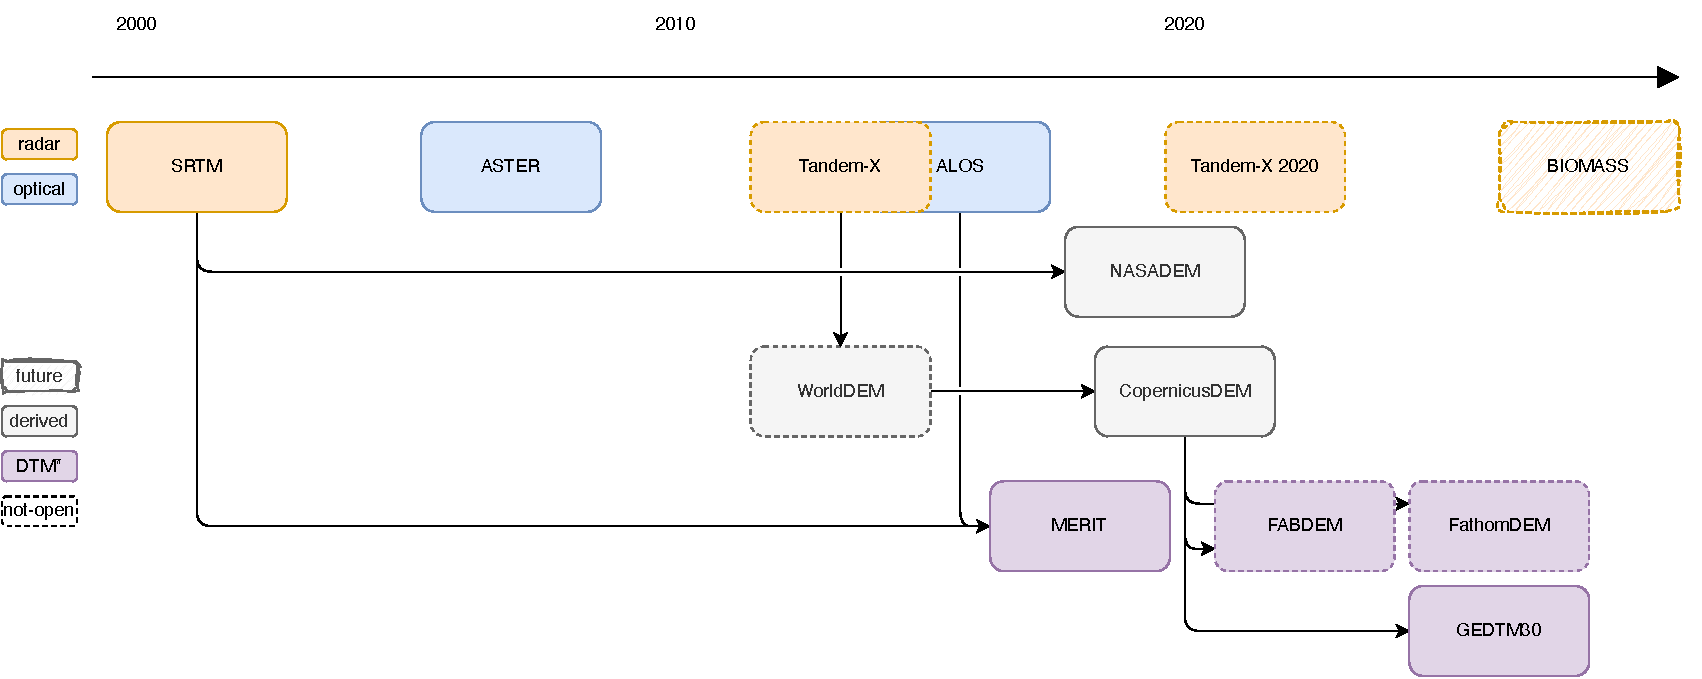
\includegraphics[width=\linewidth]{dems_overview}
  \caption{An overview of current gDEMs}%
  \label{fig:gdem_inheritance}
\end{figure*}
Note that all these products differ considerably in terms of coverage, resolution, accuracy and licensing.
Even the same product can have different versions, with different resolutions and licenses.

%

For example, SRTM is freely available,
\marginnote{SRTM}\index{SRTM}
including its derived NASADEM, and was first introduced at \qty{90}{m}, with subsequent versions at \qty{30}{m}.
Tandem-X, and its derived WorldDEM, is a commercial product, with a resolution of \qty{\pm12}{m}.
WorldDEM-NEO, a newer version of WorldDEM with more Tandem-X data (as used in Tandem-X 2020), even has a resolution of \qty{\pm5}{m}.
CopernicusDEM is a resampled WorldDEM---bought with your taxpayer money by ESA and freely distributed---at \qty{30}{m} resolution.
The pseudo DTMs FABDEM (\textbf{F}orest \textbf{A}nd \textbf{B}uilding removed) and FathomDEM, while derived from the freely available CopernicusDEM, are only free for research purposes.

Similarly, while ALOS World3D is freely available at \qty{30}{m}, it also comes in a commercial version at \qty{5}{m} resolution.
There is even a \qty{0.5}{m} commercial version, based on multiple optical satellites, available on request.

% We list only the ones available as open-access?
% For instance AW3D is also available as 5m-grid, but €€€.

% Maybe we should make our own table with paid products too? Like that table: \url{https://github.com/DahnJ/Awesome-DEM#summary}
% I find it interesting to know that some products are not free, and way better

% \usepackage{booktabs}
\begin{table*}[]
  \begin{tabular}{@{}lclllll@{}}
    \toprule
    & Year released & By                 & Sensor  & Type               & License & Resolution \\
    \midrule
    SRTM          & 2001          & NASA               & InSAR   & DSM                & Open    & 30--90m    \\
    ASTER         & 2009          & NASA               & optical & DSM                & Open    & 30m        \\
    Tandem-X      & 2014          & DLR                & InSAR   & DSM                & Closed  & 12m        \\
    WorldDEM      & 2014          & Airbus             & InSAR   & DSM/DTM$^{\prime}$ & Closed  & 5--12m     \\
    ALOS          & 2016          & JAXA               & optical & DSM                & Open    & 30m        \\
    MERIT         & 2017          & \citet{Yamazaki17} & InSAR   & DTM$^{\prime}$     & Open    & 90m        \\
    NASADEM       & 2019          & NASA               & InSAR   & DSM                & Open    & 30m        \\
    CopernicusDEM & 2020          & ESA                & InSAR   & DSM                & Open    & 30--90m    \\
    Tandem-X 2020        & 2022          & \citet{wesselNewTanDEMX20202022}   & InSAR   & DSM     & Closed  & 30m        \\
    FABDEM        & 2022          & \citet{Hawker22}   & InSAR   & DTM$^{\prime}$     & Closed  & 30m        \\
    FathomDEM        & 2025          & \citet{uheFathomDEMImprovedGlobal2025}   & InSAR   & DTM$^{\prime}$     & Closed  & 30m        \\
    GEDTM30        & 2025          & \citet{hoGEDTM30GlobalEnsemble2025}   & InSAR   & DTM$^{\prime}$     & Open  & 30m        \\
    \bottomrule
  \end{tabular}
  \caption{Overview of global DEMS, see Figure~\ref{fig:dem_comparison} for their lineage.}%
  \label{tab:gdem_overview}
\end{table*}

% TODO: A few words about fusion? [Okolie22] has very long review.

\begin{figure*}
  \centering
  \begin{subfigure}[t]
    {0.45\linewidth}
    \includegraphics[width=\linewidth]{nasadem.png}
    \caption{NASADEM}\label{fig:nasadem}
  \end{subfigure}
  \qquad
  \begin{subfigure}[t]
    {0.45\linewidth}
    \includegraphics[width=\linewidth]{copernicusdem.png}
    \caption{CopernicusDEM}\label{fig:copernicusdem}
  \end{subfigure}
  \caption{NASADEM and CopernicusDEM for the Indus delta in Pakistan. Note the striped noise in NASADEM, and how CopernicusDEM has more detail. There is $\sim$twelve years between these images.}%
  \label{fig:dem_comparison}
\end{figure*}





%%%%%%%%%%%%%%%%%%%%
%
\section{Specific characteristics of gDEMs}[Specific characteristics]

%%
\subsection{Global often means near-global}

The data collected depend on the orbit of the satellite.
Some satellites have a polar orbit and can therefore completely measure the Earth (ICESat-2 is one example, see~\ref{fig:orbit}), while some will cover only certain latitudes (\eg\ GEDI, see~\ref{fig:orbit}).

Similarly, while the Tandem-X mission produced a DEM with a global coverage, the SRTM DEM was measured from the Space Shuttle and only covers up to \qty{60}{\degree} latitude.

%%
\subsection{Format}

The formats used to store and exchange DEMs have historically been defined by the military, which are still used by many government agencies.
One example is the \emph{Digital Terrain Elevation Data} (DTED) format, developed in the 1970s, which stores elevation in integers (which tells us a lot about the accuracy and precision possible 50 years ago).
It specifies several possible \emph{levels} in terms of resolution (in arcseconds), from level 0 at \qty{\pm1}{km} to level 2 at \qty{30}{m}.
More recently, in 2016, the Defence Gridded Elevation Data (DGED) has been defined, specifying more levels to higher resolutions and allowing GeoTIFFs to used (which removes the integer constraint).
\marginnote{GeoTIFF}
DGED also defines the structure and the specific tiling of the data at higher latitudes, as resolutions in arcseconds become smaller near the poles.

%
Most of the gDEMS are tiled in a similar way.
CopernicusDEM---adhering to the DGED level 3 standard---has tiles of 3601$\times$3601 pixels on the equator, but 3600$\times$2400 (height, width) pixels at \qty{50}{\degree} latitude, 3600$\times$1800 at \qty{60}{\degree} latitude, 3600$\times$1200 at \qty{70}{\degree} latitude, becoming as small as 3600$\times$360 for the last 5 degrees of latitude.
This tiling scheme results in pixels being as square as possible, but makes it hard to work with tiles from different latitudes.

In this context it becomes clear that the resolution should not be discussed in terms of meters, but terms of degrees (or divisions of a degree).
As the Earth has a circumference of \qty{\pm40000}{km} (measured around the Equator), \ang{1} of latitude is \qty{\pm111}{km} and \ang{1} of longitude is $111\cos\phi$ \unit{km} at latitude $\phi$.
Degrees are further divided into 60 arcminutes (\lq), which themselves are divided into 60 arcseconds (\lq\lq).
In practice, the highest resolution for SRTM (\qty{30}{m}) is actually \ang{;;1}, and its \qty{90}{m} product has a resolution of \ang{;;3}.
DTED level 0 thus has a resolution of \ang{;;30}, while level 2 has a resolution of \ang{;;1}.
%

Datasets such as SRTM and NASADEM can be provided as \texttt{.hgt} (height) files, which are not even a format, but are simply a binary file with the elevation values listed in a given order, with the geographic extent to be derived from the filename.
% GDAL can however read these files.


\begin{floatbox}
\begin{kaobox-practice}[frametitle=\faCog\ Downloading gDEMs]
Most of the gDEMS are available in a standard and easily accessible format, such as GeoTIFF\@.
However, for broad compatibility, recent advances such as new compression techniques and tiling strategies are not yet widely used.
\\ \\
One such advance is Cloud Optimized GeoTIFF (COG: \url{https://www.cogeo.org}), which is a normal GeoTIFF with a specific structure that allows it to be read piecewise from the cloud.
Without such a structure, a GeoTIFF has to be downloaded in its entirety---even if one is only interested in a small part of it---before it can be read.
\end{kaobox-practice}
\end{floatbox}

%%%
\subsection{Accuracy}

The accuracy of gDEMs is often broken down into several components and related metrics, which are not always well-defined.
The DTED and DGED specifications differentiate between horizontal and vertical accuracy, and within each defines both relative and absolute accuracy.
Relative accuracy describes the consistency of the measurements, specified as the random error component of the uncertainty between two DEM pixels. % this is related to precision
Absolute accuracy describes the total error of a measurement compared to a reference.

%

The DGED standard specifies a relative vertical accuracy of less than \qty{12}{m} for level 2 (resolution of \ang{;;1}, or \qty{\pm30}{m}) and an absolute accuracy (goal) of \qty{18}{m}.
CopernicusDEM reports a mean error of less than \qty{2}{m} for 65\% of its tiles, and another 19\% with an error of less than \qty{5}{m} in terms of absolute accuracy.


%%%
\subsection{Errors}

As with any measurements taken, gDEMs contain errors and outliers.
For example, SRTM contains a lot of noise, and has (diagonal) striping artefacts, visible in Figure~\ref{fig:nasadem} for the derived NASADEM\@.

%

Another example is CopernicusDEM that suffers from multipath errors in urban areas, which lead to small pits in the DEM, see Figure~\ref{fig:copernicus_error}.
\begin{figure*}
  \centering
  \includegraphics[width=\linewidth]{low_outliers.pdf}
  \caption{Low outliers in CopernicusDEM, with orthophoto on the right for context. Electricity poles, visible by their shadows, are the cause for these errors here.}%
  \label{fig:copernicus_error}
\end{figure*}

%

Most gDEMS suffer from voids in steep terrain, as peaks can occlude valleys below (called the shadow effect).
%%\paragraph{void filling: \url{https://en.wikipedia.org/wiki/Shuttle_Radar_Topography_Mission#Void-filled_SRTM_datasets}
\marginnote{voids in DEMs}
These voids are often filled not only by interpolation, but with the help of other gDEMS, as they measured the same area from a different angle.

%

Furthermore, gDEM products are often accompanied by a quality layer, which indicates where data has been void-filled.
Similarly, error masks with the calculated instrument error and water masks are often provided alongside the elevation data.



%%
% \paragraph{integration with sea-level datasets}
%%
% \paragraph{accuracy affected by slope (most image-based products)}


%%
\subsection{Vertical datums}

Global DEMs are vertically referenced to a specific geoid, specifically EGM96 (EPSG:5171) for SRTM and EGM2008 (EPSG:3855) for CopernicusDEM\@.%
\marginnote{Earth Gravitational Model (EGM)}
Be aware that there is a small difference---generally less than \qty{0.5}{m}---between these versions of the EGM geoid.

% MSS = Geoid + MDT
Note that the geoid is not the same as the mean sea level (MSL),%
\index{mean sea level (MSL)}\marginnote{mean sea level (MSL)}
as it does not take into account the dynamic effects of temperature and currents.
Depending on the location, the difference between the geoid and MSL can be up to \qty{1.5}{m}.


%%
\subsection{gDEMs are DSM (more than DTM)}

In contrast to local DEMs, which are often provided as either a classified point cloud, or as separate raster DSMs and DTMs, gDEMs should be classified as DSMs.
The current measurement techniques will measure the top of canopy and buildings, and not the ground below.
This is the largest source of error in gDEMS, and can considerably limit the applicability of the data.

%

Several attempts have been made to correct gDEMS for vegetation and buildings, leading to what we denote as a \emph{pseudo DTM} (DTM$^{\prime}$).
\marginnote{DTM$^{\prime} =$ pseudo DTM}
While these methods improve the accuracy of gDEMs considerably, they are not perfect, and resulting terrain still contain vegetation and/or buildings.
Recent work has also suggested that while these datasets have improved vertical accuracy, the accuracy of derived geomorphometric parameters such as slope and curvature suffers.
% are still far removed from a local DTM\@.

%%%%%%%%%%%%%%%%%%%%
%
\section{Notes and comments}

Space lidar is promising as a source to reconstruct gDEMs because lidar penetrates vegetation, and thus obtaining a DTM is an easier process.
Recently, several global \emph{coastal} pseudo DTMs---covering only areas near or below sea-level---have been produced using space lidar (to some extent): CoastalDEM~\citep{Kulp24}, DiluviumDEM~\citep{Dusseau23} and DeltaDTM~\citep{Pronk24}.
Likewise, the new ESA Biomass mission~\citep{queganEuropeanSpaceAgency2019}---launched in 2025---will use P-band radar to penetrate vegetation and measure the ground below, potentially enabling a truly global DTM in the future.

\citet{Yang11} provide a detailed list of applications where gDEMs (SRTM, but when the paper was written (2011) SRTM was still the main product available globally) are necessary as input.

\citet{Schumann2018} make a case for the need for high-accuracy open-access DEMs, demonstrating SRTM is not good enough for many applications.

\citet{Hancock2021} investigates the requirements for a global lidar DEM\@.

Further reading about DEM terminology can be found in \citet{Guth2021}, which is one of the products of the \emph{Digital Elevation Model Intercomparison eXperiment} (DEMIX) group.
They also published a paper comparing the vertical accuracy and derived parameters of several gDEMs~\citep{guthRanking10Global2024}.

Arguably the best place to download DEMs (gDEMS, local ones, lidar datasets, etc.) is OpenTopography (\url{https://opentopography.org}).
Otherwise each gDEM has its own download portal, with its own registration systems and its specific ways of searching and downloading the data.
In case of the most recent gDEMS, such as CopernicusDEM, the data must be downloaded as \texttt{.tar} (archives) for \ang{1}$\times$\ang{1} tiles via FTP, in folders for each continent and then country.
Data is duplicated for the border areas, totalling \qty{2}{TB}.

To learn more about the DGED format, read \url{https://dgiwg.org/documents/dgiwg-standards}.
Similarly, reading a user guide on any of the gDEMS is a good idea, such as the one for \href{https://spacedata.copernicus.eu/documents/20126/0/GEO1988-CopernicusDEM-SPE-002_ProductHandbook_I3.0+%281%29.pdf}{CopernicusDEM Product Handbook}.

\citet{Hawker22} give the details how the vegetation and buildings are removed from CopernicusDEM to create FABDEM\@.

%%%%%%%%%%%%%%%%%%%%
%
\section{Exercises}

% TODO: think of some exam questions to put here
\begin{enumerate}
  \item How wide is 1 degree longitude at the latitude where the city of Delft is? And at the North Pole?
  \item How old is the oldest gDEM, and what latitudes did it cover?
  \item Assume you want to compare the elevations from AHN5 to those of CopernicusDEM\@. Which steps/conversions are needed?
\end{enumerate}
